\documentclass[a4paper,10pt]{article}

\usepackage[utf8]{inputenc}
\usepackage[OT4]{polski}
\usepackage{amsmath, amsthm, amssymb}
\usepackage{hyperref}
\usepackage{graphicx}
\usepackage[margin=2.5cm]{geometry}

\begin{document}

\tableofcontents

\section{Relacja klasyfikacji}
Jako $D$ oznaczamy pewien skończony zbiór obiektów. W tym zbiorze wprowadzimy dwuargumentową relację $R$. Relacja $R$ nazywana jest relacją klasyfikacji, jeśli spełnia dwa warunki:
\begin{enumerate}
 \item Relacja $R$ dzieli zbiór $D$ na podzbiory $D_i$ tak, że każdy dowolony element $D$ należy do jednego podzbioru $D_i$:
\begin {equation}
 \displaystyle\mathop{\forall}_{x \in D} \mathop{\exists}_i x \in D_i
\end {equation}
\begin{equation}
 D = \sum_i D_i
\end{equation}
 \item Iloczyn dwóch podzbiorów jest zbiorem pustym. Każdy element zbioru $D$ należy więc tylko do jednego podzbioru $D_i$:
\begin{equation}
 \mathop{\forall}_{i, j, i \neq j} D_i \cap D_j = \emptyset
\end{equation}
\end{enumerate}

\section{Zadanie rozpoznawania. Elementy składowe rozpoznawania}
\subsection{Zadanie rozpoznawania}
Celem zadania rozpoznawania jest zbudowanie algorytmu $A$ realizującego odwzorowanie (klasyfikację + przypisanie etykiet):
\begin{equation}
 A : D \rightarrow I \cup \{i_{\emptyset}\}
\end{equation}
który przypisuje do każdego elementu zbioru $D$ etykietę (numer klasy) należącą do zbioru $I \cup \{i_{\emptyset}\}$, gdzie $i_{\emptyset}$ jest odpowiedzią ,,nie wiem''. Dobry algorytm charakteryzuje się małą liczbą odpowiedzi ,,nie wiem''.

Dopuszczalny jest wariant, w którym identyfikujemy czy obiekt należy do sumy niektórych podzbiorów, np. $p \in D_1 \cup D_2$

Interesują nas takie relacje, które generują skończoną liczbę klas (relacja ta jedynie dzieli zbiór obiektów na podzbiory, ale nie przypisuje im etykiet).

\subsection{Elementy składowe rozpoznawania}
Odwzorowanie $A$ jest realizowane jako złożenie trzech odwzorowań
\begin{equation}
 A = F \cdot C \cdot B
\end{equation}
\begin{enumerate}
 \item Recepcja\footnote{Nie mylić z incepcją}:
    \begin{equation}
      B: D \rightarrow X
    \end{equation}
 \item Funkcja przynależności:
    \begin{equation}
      C: X \rightarrow R^L, R^L \rightarrow R^I
    \end{equation}
  \item Proces podejmowania decyzji:
    \begin{equation}
      F: R^I \rightarrow I \cup \{i_{\emptyset}\}
    \end{equation}
\end{enumerate}

\section{Recepcja cech. Zasada Brawermanna.}
Recepcja jest to arbitralne przypisane obiektowi zestawu cech w postaci wektora $X = [x_1, x_2, x_3, \ldots, x_L]$, $X \in R^L$, gdzie $L$ jest liczbą parametrów. \ref{fig:brawermann}

Obrazując, zasada Brawermanna mówi, że wartości $L_i$ należy maksymalizować, a $D_j$ minimalizować.

\begin{figure}[ht]
  \centering
  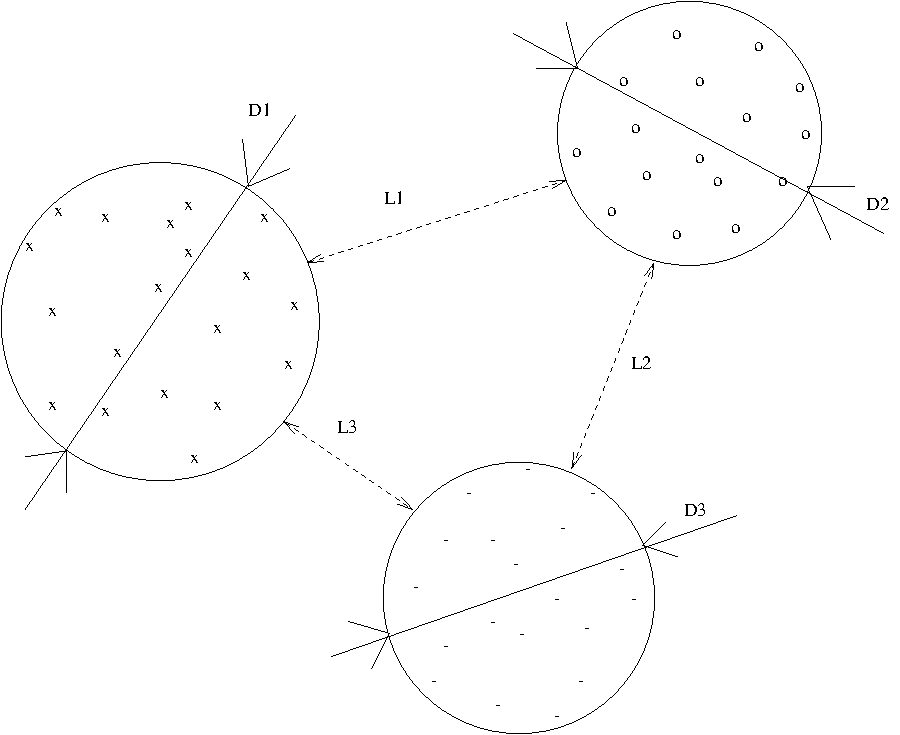
\includegraphics[width=\textwidth]{brawermann.pdf}
  \caption{Zasada Brawermanna}
  \label{fig:brawermann}
\end{figure}

Każda zmienna wektora może być zmienną liczbową lub jakościową. Trudność polega na takim doborze cech, by wybrać tylko te najistotniejsze, zazwyczaj opieramy się o wynik symulacji, wcześniejsze doświadczenia lub intuicję.

Przy wyborze przestrzeni cech nalęzy kierować się zasadą Brawermanna, która mówi, że obiekty jednej klasy powinny w przestrzeni cech tworzyć skupiska możliwie maksymalnie zwarte wewnętrznie i możliwie najbardziej oddalone od podobnych skupisk dla innych klas.

\section{Odwzorowanie: funkcja przynależności.}
Realizacja odwzorowania $C$ polega na określeniu wartości podobieństwa pomiędzy rozpoznawanym obiektem $\overrightarrow{a}$ $(\overrightarrow{a} \in R^L)$ i obiektami z klasy $D_i: C^i(\overrightarrow{a})$. Dla obiektu $\overrightarrow{a}$ określamy jego podobieństwo do klasy $D_i = 1, 2, \ldots, I$

$C^i(\overrightarrow{a})$ zależy od stosowanej metody.

\section{Odwzorowanie: podejmowanie decyzji.}
Podejmowanie decyzji realizujemy na podstawie wartości funkcji przynależności. W najprostszym przypadku $\overrightarrow{a}$ przypisujemy do tej klasy, dla której mamy dominującą wartość funkcji przynależności. Przy podejmowaniu decyzji warto zadbać, aby wartość maksymalna funkcji przynależności miała charakter naprawdę maksymalny:
\begin{equation}
C^{i_{max}}(\overrightarrow{a}) \geq r \sum_{i \neq i_{max}} C^i(\overrightarrow{a})
\end{equation}
\begin{equation}
 0.5 \leq r \leq 1
\end{equation}

Jeśli ten warunek nie jest spełniony to odpowiedz ,,nie wiem''.

\section{Rozpoznawanie a klasyfikacja. Ogólny schemat rozpoznawania.}
W zadaniu rozpoznawania \textit{a priori} znana jest klasyfikacja, a zadanie rozpoznawania właśnie polega na tym, żeby określić, czy nowy obiekt należy do jednej ze znanych klas tzn. że klasyfikacja i rozpoznanie są to różne zadania, które możemy rozwiązać za pomocą różnych metod.
Ogólny schemat rozpoznawania: \ref{fig:recognition}

\begin{figure}[ht]
  \centering
  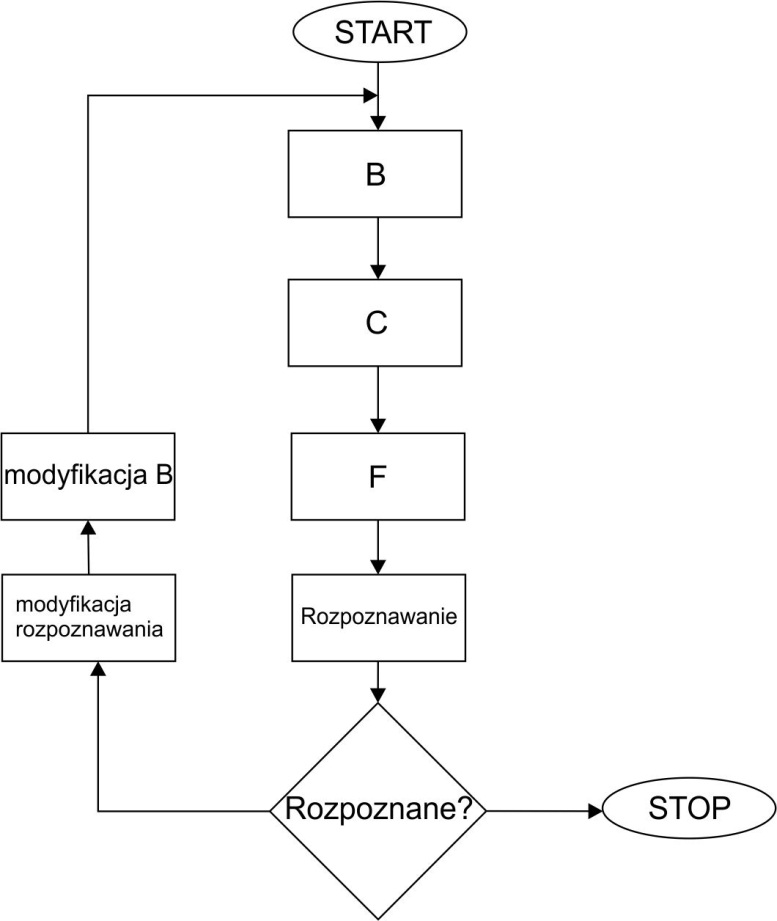
\includegraphics{rozpoznawanie.png}
  \caption{Rozpoznawanie}
  \label{fig:recognition}
\end{figure}

W ogólnym przypadku rozpoznawanie jest procesem iteracyjnym.

\section{Metody minimalnoodległościowe. Wybór metryki.}
Wybór właściwej metryki musi być dopasowany do zasady Brawermana i zwykle realizowany jest empirycznie metodą prób i błędów albo całkowicie arbitralnie.

Definicja:
Metryka $\varphi(w)$ w przestrzeni $X$ jest odwzorowaniem, które spełnia założenia:
\begin{enumerate}
 \item \begin{equation}
         \mathop{\forall}_{\overrightarrow{x}, \overrightarrow{y} \in X} \varphi(\overrightarrow{x}, \overrightarrow{y}) \geq 0, \; \, \: \varphi(\overrightarrow{x}, \overrightarrow{y}) \in R^{+}
       \end{equation}
 \item \begin{equation}
         \mathop{\forall}_{\overrightarrow{x} \in X} \varphi(\overrightarrow{x}, \overrightarrow{x}) = 0
       \end{equation}
 \item \begin{equation}
         \mathop{\forall}_{\overrightarrow{x}, \overrightarrow{y} \in X} \varphi(\overrightarrow{x}, \overrightarrow{y})  = \varphi(\overrightarrow{y}, \overrightarrow{x})
       \end{equation}
 \item \begin{equation}
         \mathop{\forall}_{\overrightarrow{x}, \overrightarrow{y}, \overrightarrow{z} \in X} \varphi(\overrightarrow{x}, \overrightarrow{y})  + \varphi(\overrightarrow{y}, \overrightarrow{z}) \geq \varphi(\overrightarrow{x}, \overrightarrow{z})
       \end{equation}
\end{enumerate}
\subsection{Metryka euklidesowa}
\begin{equation}
  \varphi_E(\overrightarrow{x}, \overrightarrow{y}) = \sqrt{\sum_{i = 1}^n (x_i - y_i)^2}
\end{equation}
\subsection{Metryka uliczna/manhattan/taksówkarza}
\begin{equation}
  \varphi_U(\overrightarrow{x}, \overrightarrow{y}) = \sum_{i = 1}^n |x_i - y_i|
\end{equation}
\subsection{Metryka Pafnutija Lwowicza Czebyszewa}
\begin{equation}
  \varphi_C(\overrightarrow{x}, \overrightarrow{y}) = \mathop{\mbox{max}}_{1 \leq i \leq n} |x_i - y_i|
\end{equation}
\subsection{Metryka Minkowskiego}
\begin{equation}
  \varphi_M(\overrightarrow{x}, \overrightarrow{y}) = \left({\sum_{i = 1}^n |x_i - y_i|^p}\right)^{\frac{1}{p}}
\end{equation}
Jeśli $p = 2$, to metryka przechodzi w metrykę euklidesową; jeśli $p = 1$ to metryka przechodzi w metrykę uliczną; jeśli $p \rightarrow \infty$, to metryka przechodzi w metrykę Pafnutija Lwowicza Czebyszewa.

\section{Metoda najbliższego sąsiada NN.}
Mając wektor cech dla badanej próbki i znając wektory cech dla próbek treningowych należy obliczyć (wg wybranej metryki) odległość badanego wektora do wszystkich wektorów treningowych. Za klasę badanego wektora uznajemy klasę jaką miał wektor, którego odległość jest najmniejsza. Jest on więc najbliższym sąsiadem.\footnote{tu można jeszcze rąbnąć rysunek}
Bardziej formalnie: Należy wybrać jako rozpoznanie $i \in I$ tę klasę, do której należy obiekt $x^{i,k} \in U$ najbliższy (w myśl przyjętej metryki $\varphi$) rozpoznanemu obiektowi $d$ (a dokładniej reprezentującemu go wektorowi $\overrightarrow{x}$).

\section{Metoda $\alpha$NN}
Istotną wadą metody NN jest przypadek, kiedy jeden z elementów istniejących klas obarczony jest błędem. W takim wypadku przydatna okazuje się metoda $\alpha$NN.
\begin{enumerate}
\item Szukamy odległości pomiędzy obiektem $\overrightarrow{a}$, a wszystkimi elementami wszystkich klas $\varphi(\overrightarrow{a},\overrightarrow{x^{i,k}})=dm$ gdzie $k = 1, 2, \ldots, L$; $i = 1,2, \ldots, I_k$; $L$ – liczba klas, $I_k$ – liczba elementów $k$-tej klasy, $m=1,2,\ldots,|D|$
\item Sortujemy $dm$ w porządku niemalejącym. Otrzymujemy $rm$, $m = 1,2,\ldots, |D|$
\item Wybieramy $\alpha$ pierwszych elementów ciągu $rm$
\item Obiekt $\overrightarrow{a}$ klasyfikujemy do klasy przedstawicieli której jest najwięcej wybranych w kroku 3
\end{enumerate}

\section{Metoda jnNN. Relacja pomiędzy metodami $\alpha$NN i jnNN.}
Istota metody jnNN polega na tym, że w określeniu funkcji przynależności bierze udział jn-ty najbliższy sąsiad. Teoretycznie wiadomo, że jeśli $jn=\frac{d+1}{2}$ to metody jnNN oraz $\alpha$NN są równoważne. Jednak w praktyce $\alpha$NN ma przewagę.

\section{Metoda wzorców. Ogólny schemat.}
Metoda ta opiera się na opracowaniu wzorca dla każdej klasy. W najprostszym przypadku wzorcami możemy określić wszystkie obiekty ciągu uczącego. W metodach tych decyzje podejmujemy w bardzo prosty sposób:

\begin{equation}
 C^i(\overrightarrow{a}) = 
\begin{cases} 1 & \mbox{gdy }\overrightarrow{a} = \{w_i\}\\
 0 & \mbox{gdy }\overrightarrow{a} \neq \{w_i\}
\end{cases}
\end{equation}

$\overrightarrow{a}$ - nowy obiekt

$w_i$ - wzorzec klasy $i$-tej

Takie metody wydają się być bardzo proste jednakże przy takim podejściu gwałtownie rośnie liczba decyzji ,,nie wiem''.
Naprostszym rozwiązaniem tego problemu jest zwiększenie ilości wzorców poprzez interpolację. Po prostu wprowadzenie ,,drobniejszej siatki wzorców''.

\section{Metoda wzorców. Wzorzec uogólniony.}
Należy określić jeden element klasy, który będzie wzorcowy. 
\begin{equation}
  \overrightarrow{m_i} = \frac{1}{I_i} \sum_{k=1}^{L_i} \overrightarrow{x^{i,k}}
\end{equation}

Fizyczną interpretacją średniej arytmetycznej jest środek ciężkości.
\begin{equation}
 C^i(\overrightarrow{a}) = 
\begin{cases} 1 & \mbox{gdy }\overrightarrow{a} = \{m_i\}\\
 0 & \mbox{gdy }\overrightarrow{a} \neq \{m_i\}
\end{cases}
\end{equation}
I korzyści będzie z tego jeszcze mniej, bo liczba decyzji będzie gwałtownie rosła. Dlatego należy wprowadzić:
\begin{equation}
C^i(\overrightarrow{a}) = \frac{1}{\delta(\overrightarrow{a_i}, \overrightarrow{m_i}) + \varepsilon_i}\mbox{, }    \varepsilon_i > 0 
\end{equation}
Jest to uproszczony, zmodyfikowany wariant metody najbliższego sąsiada, w której rolę najbliższego sąsiada spełnia moda.
Nie jest to w żadnym wypadku recepta na sukces. Może być taka sytuacja, że moda jednej klasy będzie leżeć bardzo blisko mody innej klasy.

\section{Metoda wzorców: otoczenia kulistyczne.}
Dla każdego elementu należy wprowadzić otoczenie kulistyczne:

\begin{equation}
 C^i(\overrightarrow{a}) = 
\begin{cases} 1 & \mbox{gdy $|\overrightarrow{a} - w^{i,k}| \leq \varepsilon^{i,k}$}\\
 0 & \mbox{w przeciwnym przypadku}
\end{cases}
\end{equation}

$\varepsilon^{i,k}$ jest to promień otoczenia kulistycznego $w^{i,k}$, w tym przypadku zakładamy, że każda klasa posiada zbiór wzorców, zatem możliwy jest przypadek, że w tym zbiorze są wszystkie obiekty klasy (skrajnie ogólny przypadek), Może również wystąpić przypadek w którym do zbioru wzorców należy tylko jeden obiekt - moda.
Warto rozważyć sytuację utworzenia obszaru (otoczki) tworzonej poprzez połączenie otoczeń kulistycznych wszystkich wzorców, wtedy podejmowanie decyzji jest bardzo proste - sprawdzamy czy nowy obiekt należy do podprzestrzenii ograniczonej tą otoczką czy też nie.

\section{Metoda funkcji potencjałowej}
Metody minimalnoodległościowe można rozwinąć w kierunku prowadzenia ,,nieliniowej metryki''.

Oznacza to, że odległość między punktem $\overrightarrow{x}$ i $\overrightarrow{y}$

\begin{equation}
|\overrightarrow{x} - \overrightarrow{y}| = |\overrightarrow{x} - \overrightarrow{z}| + |\overrightarrow{z} - \overrightarrow{y}|
\end{equation}

Taką nieliniowość wprowadzamy w celu nadania nieliniowo większej wagi obiektom znajdującym się bliżej obiektu ocenianego, ew. odwrotnie. Typową sytuacją korzystania z przestrzeni rozciągniętej jest sytuacja, kiedy skupiska tworzące klasy są blsko siebie. Należy wprowadzić taką miarę, żeby te skupiska rozciągnęła i oddaliła od siebie. Taka potrzeba np. zachodzi w metodach aproksymacyjnych w których zwykle od przestrzeni $R_n \rightarrow R_m$ i $m \ll n$\footnote{niech ktoś to zweryfikuje}, to znaczy w metodach istotnie redukujących wymiar przestrzeni cech.

Funkcja potencjałowa
Potencjał pomiędzy punktami $\overrightarrow{x}$ i $\overrightarrow{y}$ proporcjonalny jest do kwadratu odległości.
\begin{equation}
p = \frac{c}{l_2}
\end{equation}
\begin{equation}
\rho(\overrightarrow{a}, \overrightarrow{x}) \rightarrow \rho^2(\overrightarrow{a}, \overrightarrow{x}) \rightarrow f(\rho^2(\overrightarrow{a}, \overrightarrow{x}))
\end{equation}
Wybór rodzaju funkcji IF należy wykonać arbitralnie.

\section{Klasyfikacja. Metoda najmniejszych przedziałów}
Załóżmy, że mamy dwie klasy, ich klasyfikacja opiera się tylko o jedną cechę:

$w$ - wzrost

klasy:

$D_1$ - europejczycy

$D_2$ - azjaci

dla każdej klasy na osi zaznaczamy wszystkie obiekty \ref{fig:min_dist}
\begin{figure}[ht]
  \centering
  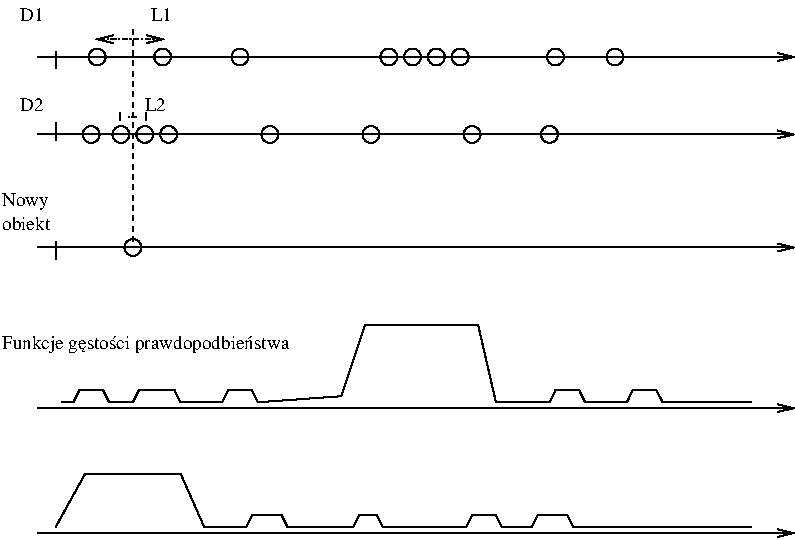
\includegraphics[width=\textwidth]{min_przed.pdf}
  \caption{Metoda najmniejszych przedziałów}
  \label{fig:min_dist}
\end{figure}

Wybieramy klasę, w której odlegości $L$ są najmniejsze. Można tę metodę przedstawić także jako metodę 2NN.
W przypadku gdy obiekt jest w $R^2$ metoda najmniejszych przedziałów staje się metodą najmniejszego pola, a w $R^3$ metodą najmniejszych objętości.

\section{Klasyfikacja. Metoda naiwnego klasyfikatora Bayesa.}
Ogólnie:
\begin{equation}
C^i(\overrightarrow{w})=P_{D_i}(w)=P(\overrightarrow{w}|D_i)
\end{equation}
Wadą tego wzoru jest, że nie bierzemy pod uwagę prawdopodobieństwa wystąpienia klasy $D_i$, które to prawdopodobieństwo w przypadku skończonego ciągu uczącego obliczone jest bardzo prosto:
\begin{equation}
P(D_i)=\frac{|D_i|}{|D|}=\frac{\mbox{liczba elementów $D_i$}}{\mbox{ogólna liczba elementów ciągu uczącego}}
\end{equation}

Wtedy:
\begin{equation}
C^i(\overrightarrow{w})=P(\overrightarrow{w}|D_i)P(D_i),\; i=1,2,\ldots,L
\end{equation}
pod warunkiem, że elementy ciągu uczącego naprawdę zostały wybrane losowo.
Ten wzór można zmodyfikować zakładając \textit{a priori} różne modele prawdopodobieństwo np. $P(D_i)$ = stała, $P(\overrightarrow{w}|D_i)$ są rozkładem normalnym
i uzyskać pod te warunki wzory.

\section{Grupowanie. Algorytm grupowania k-średnich.}
Kroki:
\begin{enumerate}
\item Określić na ile grup $k$ powinien być podzielony zbiór obiektów $D$
\item Losowo przypisz $k$-obiektów z $D$: $\overrightarrow{m_1}, \overrightarrow{m_2}, \overrightarrow{m_3}, \ldots, \overrightarrow{m_k}$ jako środki odpowiednio $D_1, D_2, D_3, \ldots, D_k$,
\item Przypisz każdy z pozostałych obiektów do grupy z minimalną odległością do środka grupy
\item Dla każdej grupy oblicz nową wartość centrum ciężkości (centroid)
\begin{equation}
\overrightarrow{m_i} = \frac{1}{I_i} \sum_{p=1}^{I_i} d_p^{(i)}
\end{equation}
gdzie:
$i=1,2,3,\ldots,k$

$I_i$ - liczba elementów w grupie

$D_i$ - zbiór elementów: $D_i = \{d_p^{(i)}, p = 1,2,3,\ldots,I_i\}$
\item Powtarzaj kroki 3-4 aż do zbieżności lub zakończenia.
\end{enumerate}

Algorytm kończy się gdy środki ciężkości już się nie zmieniają.
Działanie algorytmu można zakończyć również za pomocą kryterium braku istotnego zmniejszenia sumarycznego błędu kwadratowego 
\begin{equation}
SSE = \sum_{i=1}^{k} \sum_{p=1}^{I_i}\rho^2 (d_p^{(i)})
\end{equation}

Algorytm nie gwarantuje znalezienia globalnego minimum SSE i zwykle daje minimum lokalne. Dlatego zaleca się aby uruchomić go kilkakrotnie z różnymi środkami początkowymi grup.

\section{Grupowanie. Metoda pojedynczego połączenia.}
Startowo uważamy, że każdy obiekt tworzy niezależną grupę.
Grupowanie realizujemy łącząc do jednej grupy obiekty oddalone o określoną odległość np. 1.
Metoda ta poszukuje minimalnej odległości pomiędzy dowolnymi rekordami z dwóch grup.

\section{Grupowanie. Metoda całkowitego połączenia.}
Startowo uważamy, że każdy obiekt tworzy niezależną grupę.
Metoda ta chce zminimalizować odległość pomiędzy obiektami z dwóch grup, które są najbardziej oddalone od siebie.

\section{Momenty obiektu.}
Niech dana będzie funkcja obiektu:
\begin{equation}
 I(x_i, y_i) \in 
\begin{cases}
 \{0, 1\} & \mbox{dla obrazów binarnych}\\
 \left[0, 1\right] & \mbox{dla obrazów w skali szarości}
\end{cases}
\end{equation}

Niech $M$, $N$, będą wymiarami obrazu oraz dany będzie współczynnik:
\begin{equation}
  \mu_{00} = \sum_{i=1}^{M} \sum_{j=1}^{N} I(x_i, y_i)
\end{equation}

Moment pierwszego rzędu - współrzędne środka ciężkości:
\begin{equation}
  \overrightarrow{x} = \mu_{10} = \frac{1}{\mu_{00}} \sum_{i=1}^{M} \sum_{j=1}^{N} x_i I(x_i, y_i)
\end{equation}

\begin{equation}
  \overrightarrow{y} = \mu_{01} = \frac{1}{\mu_{00}} \sum_{i=1}^{M} \sum_{j=1}^{N} y_i I(x_i, y_i)
\end{equation}

Momenty drugiego rzędu - bezwładność obiektu
\begin{equation}
  \mu_{20} = \frac{1}{\mu_{00}} \sum_{i=1}^{M} \sum_{j=1}^{N} (x_i - \overline{x})^2 I(x_i, y_i)
\end{equation}
\begin{equation}
  \mu_{22} = \frac{1}{\mu_{00}} \sum_{i=1}^{M} \sum_{j=1}^{N} (y_i - \overline{y})^2 I(x_i, y_i)
\end{equation}
\begin{equation}
  \mu_{11} = \frac{1}{\mu_{00}} \sum_{i=1}^{M} \sum_{j=1}^{N} (x_i - \overline{x})(y_i - \overline{y}) I(x_i, y_i)
\end{equation}

Wykorzystanie momentów do obliczenia innych parametrów obiektu:
\begin{itemize}
 \item kierunek prostokąta granicznego
 \begin{equation}
   \Theta = \arctan \left(\frac{2 \mu_{11}}{\mu_{20} - \mu{02}}\right)
 \end{equation}
\end{itemize}

\section{Momenty konturu.}
Niech kontur obiektu składa się z $N$ pikseli. 
Niech $d(i),\; i=1,2,\ldots,N$ będzie euklidesową odległością $i$-tego piksela od środka ciężkości obiektu.

\begin{enumerate}
\item Jednowymiarowe momenty konturu rzędu $p$:

\begin{equation}
m_p = \frac{1}{N} \sum_{i=1}^{N} d^p(i)
\end{equation}

\begin{equation}
\mu_p = \frac{1}{N} \sum{i=1}^{N} (d(i) - m_1)^p
\end{equation}

\item Forma znormalizowana:

\begin{equation}
\overrightarrow{m_p} = \frac{\overrightarrow{m_p}}{\gamma},\;\; \overrightarrow{\mu_p} = \frac{\overrightarrow{\mu_p}}{\gamma}, \;\; \mbox{gdzie } \gamma = (\mu_2)^{\frac{p}{2}}
\end{equation}
\end{enumerate}


\end{document}
